\chapter{Architecture}

In this chapter will be discussed deeply the architecture of the three main parts of the perceptron. The general structure could be summarized by the following schema:
\begin{figure}[H]
	\centering
	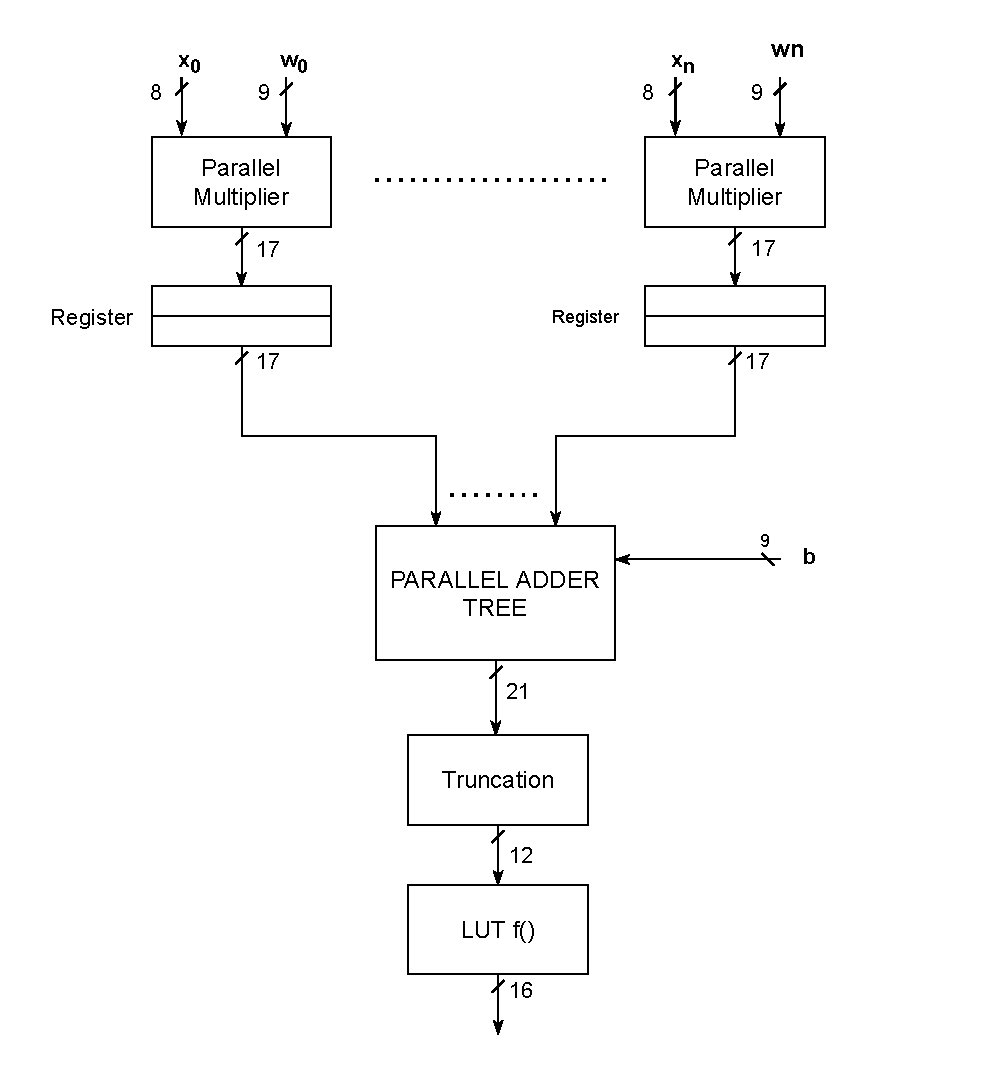
\includegraphics[width=12cm]{img/architecture_general_schema.pdf}
	\caption{General Schema}
\end{figure}

\section{Multiplication Circuit Architecture}
The Multiplication Circuit, as said before, will be implemented through a Parallel Multiplier. The inputs $b_{i}$ and $w_{i}$ are composed respectively by $b_{x} = 8$ bits and $b_{w} = 9$ bits. In the following image is presented the architecture with these particular inputs.
\begin{figure}[H]
	\centering
	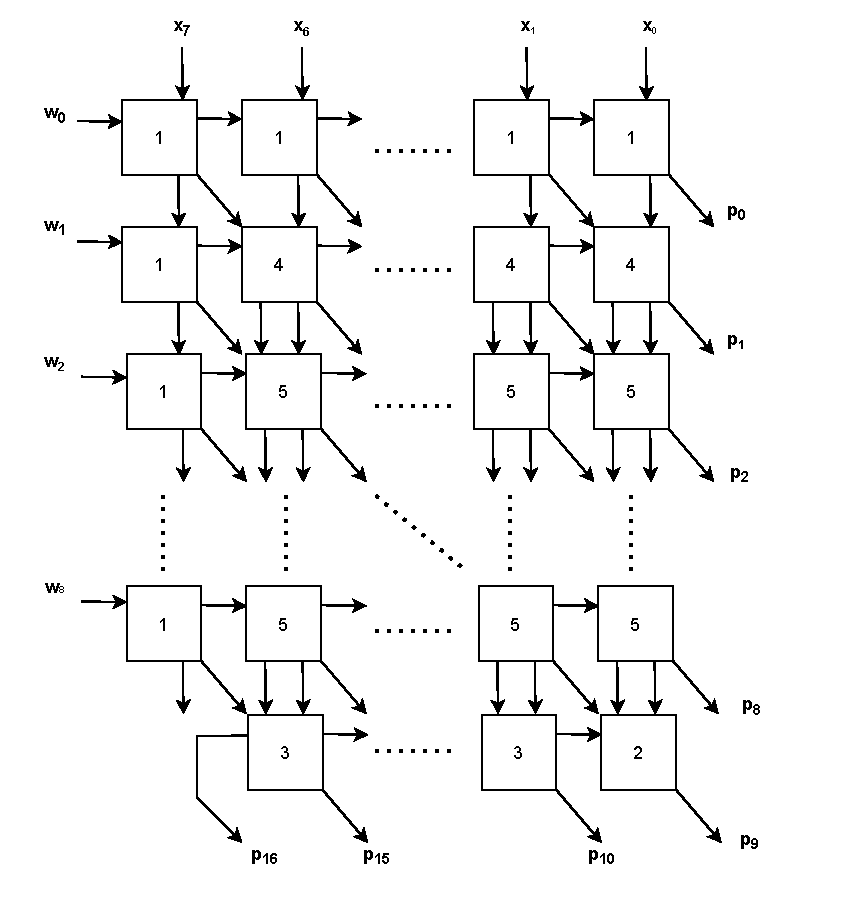
\includegraphics[width=13cm]{img/architecture_parallel_multiplier.pdf}
	\caption{Parallel Multiplier Architecture}
\end{figure}
\section{Adder Circuit Architecture}
In order to compute the equation (1.1) different sums need to be computed. The building block of this part will be the \textbf{Parallel Adder with Pipeline}: as said before, by adding some registers in between the Carry chains, the critical path impact can be reduced. Furthermore, by exploiting the parallel architecture, a single sum can be computed in a single clock cycle. In the next figure will be presented the Parallel Adder:
 \begin{figure}[H]
 	\centering
 	\makebox[\textwidth][c]{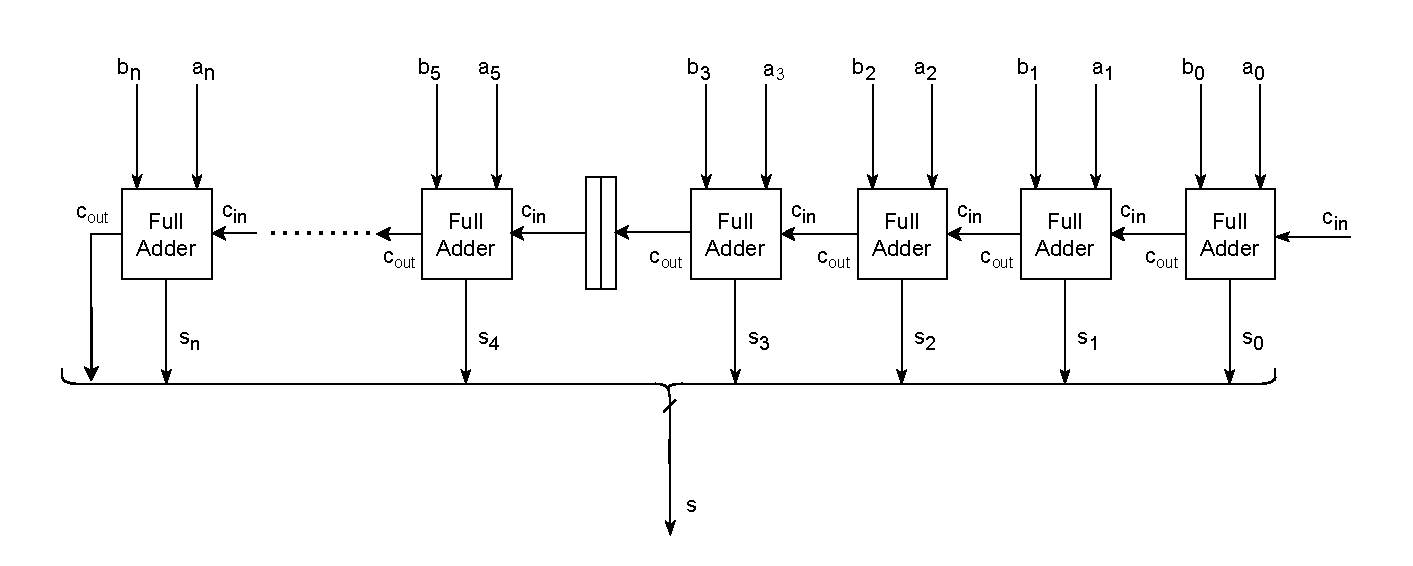
\includegraphics[width=1.5\textwidth]{img/architecture_full_adder_with_pipeline.pdf}}%
 	\caption{Parallel Adder Architecture}
 \end{figure}
To implement the whole sum of 11 terms, in order to decrease the number of cycles needed to compute the whole sum and to reduce the number of bits needed, a tree approach has been chosen. The schema of the tree parallel adder is the following:
\begin{figure}[H]
	\centering
	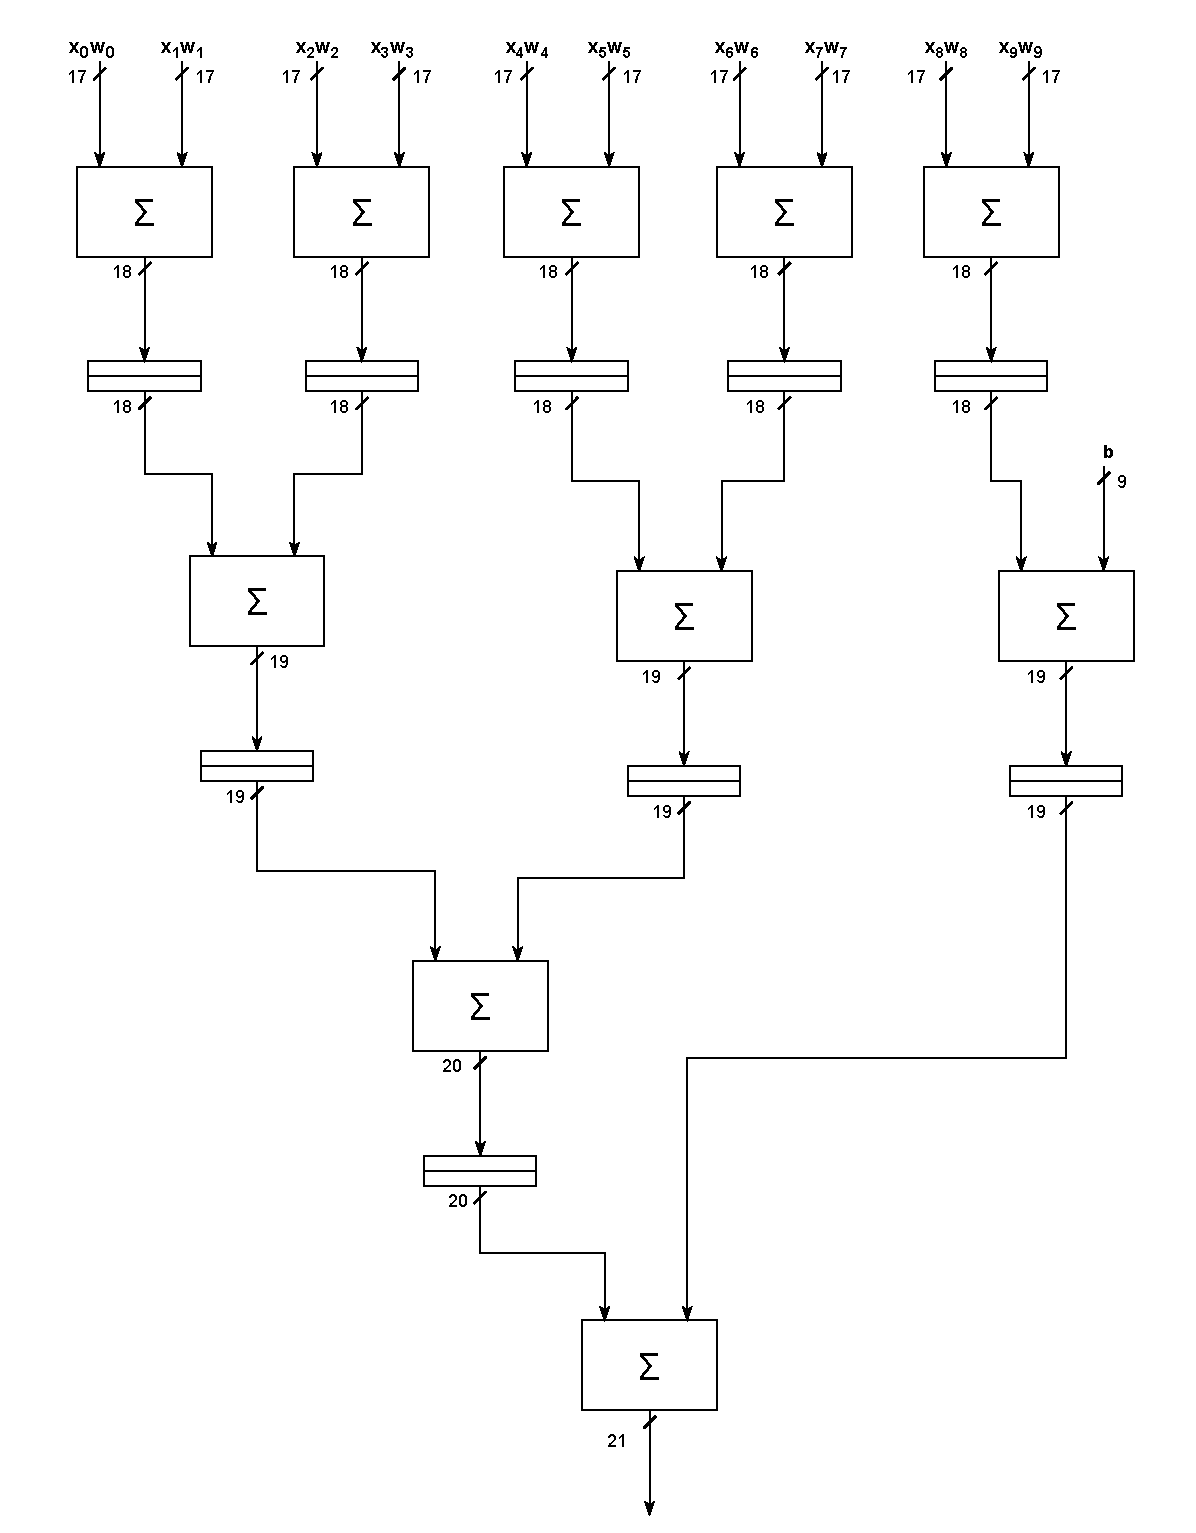
\includegraphics[width=\textwidth]{img/architecture_adder_tree.pdf}
	\caption{Parallel Multiplier Architecture}
\end{figure}

Some register has been put in between the sum to limit the critical path impact on the performances and clock period limit.
\section{Activation Function Circuit Architecture}
At the end of the computation of the latter phase the output is composed by $21$ bits. The computation of the sigmoid function will be done through a \textbf{Look-Up-Table}, which will need \textbf{$2^{21} = $2097152 entries} of different outputs with $16$ bits. In order to reduce the size of the Look-Up-Table a truncation is needed: from $21$ bits to $12$ bits. In this case the Look-Up Table will be composed by \textbf{$2^{12} = $4096 entries}, but, by exploiting the \textbf{odd symmetry} of the sigmoid, only \textbf{$4096/2 = $ 2048 entries} are needed.
\begin{figure}[H]
	\centering
	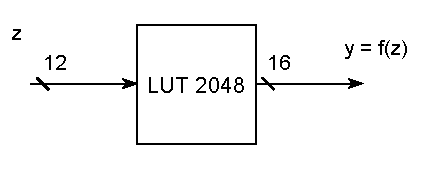
\includegraphics[width=0.6\textwidth]{img/architecture_lut_optimized.pdf}
	\caption{Look-Up Table Architecture}
\end{figure}
 